\documentclass{article}
\usepackage{amsmath}
\usepackage{graphicx}
\usepackage{geometry}
\usepackage{amsfonts}
\usepackage{amssymb}
\usepackage{graphicx}
\usepackage[utf8]{inputenc} %Spanish input                                      
\usepackage[T1]{fontenc} % Use 8-bit encoding that has 256 glyphs 
\usepackage[spanish, es-tabla]{babel}        
\usepackage{float}
\usepackage{lscape}
\usepackage{enumerate}
\usepackage{color}
\usepackage{algpseudocode}
\usepackage{mathtools}
\usepackage{wrapfig}
\usepackage{subfig}
\usepackage{cite} % para contraer referencias
\usepackage[hidelinks]{hyperref}
\usepackage{xstring}
\usepackage{listings}
\usepackage{lipsum}
\usepackage{courier}
\usepackage{fancyhdr}
\usepackage[ruled,vlined,linesnumbered]{algorithm2e}
\usepackage{setspace}


%------------------------------------------------------------------------
\newtheorem{theorem}{Theorem}
\newtheorem{acknowledgement}[theorem]{Acknowledgement}
%\newtheorem{algorithm}[theorem]{Algorithm}
\newtheorem{axiom}[theorem]{Axiom}
\newtheorem{case}[theorem]{Case}
\newtheorem{claim}[theorem]{Claim}
\newtheorem{conclusion}[theorem]{Conclusion}
\newtheorem{condition}[theorem]{Condition}
\newtheorem{conjecture}[theorem]{Conjecture}
\newtheorem{corollary}[theorem]{Corollary}
\newtheorem{criterion}[theorem]{Criterion}
\newtheorem{definition}[theorem]{Definition}
\newtheorem{example}[theorem]{Example}
\newtheorem{exercise}[theorem]{Exercise}
\newtheorem{lemma}[theorem]{Lemma}
\newtheorem{notation}[theorem]{Notation}
\newtheorem{problem}[theorem]{Problem}
\newtheorem{proposition}[theorem]{Proposition}
\newtheorem{remark}[theorem]{Remark}
\newtheorem{solution}[theorem]{Solution}
\newtheorem{summary}[theorem]{Summary}
\newenvironment{proof}[1][Proof]{\textbf{#1.} }{\ \rule{0.5em}{0.5em}}
\pagestyle{fancy}
\setlength{\textwidth}{7.0in}
\setlength{\oddsidemargin}{-0.35in}
\setlength{\topmargin}{-0.5in}
\setlength{\textheight}{9.0in}
\setlength{\parindent}{0.3in}
\setlength{\pdfpagewidth}{88.184mm}
\setlength{\pdfpageheight}{113.854mm}
\setlength{\footskip}{12.0pt}


\newcommand{\thelink}{\@empty}
\newcommand{\link}[2]{%
  \IfSubStr{#1}{:}{\renewcommand\thelink{#1}}{\renewcommand\thelink{#1:#2}}%
  \href{\thelink}{\texttt{#2}}%
}
%--------------------------------------------------------------
\geometry{
  a4paper,
  left=30mm,
  right=30mm,
  headheight=3cm,
  top=2.5cm,
  bottom=3.5cm,
  footskip=0cm
}
\begin{document}[\normalsize]
\begin{titlepage}
	\title{BIOGEOGRAPY BASED OPTIMIZATION}
	\author{Pablo Huertas Arroyo}
	\date{ \today }


	\maketitle
	\begin{figure}[h]
		\centering
		
\includegraphics[scale=4]{LogoUGR.png}
	\end{figure}


	\hspace{-1.7cm}
	\newline Correo: \link{mailto}{phuertas@correo.ugr.es}
	\newline DNI:77033078Y
	\newline Grupo 3A, subgrupo 2
\end{titlepage}

\newpage
\tableofcontents


\newpage
\section{\large RESUMEN}
\subsection{\normalsize Algoritmo BBO}\large
El algoritmo BBO (Biogeography Based Optimization) es un algoritmo evolutivo que optimiza una funcion
de forma estocastica e iterativa mejorando las soluciones candidatas con respecto a una medida de calidad
llamado fitness.\\

BBO optimiza un problema manteniendo una poblacion de soluciones candidatas(elitismo), y creando nuevas soluciones con dos procesos
llamados migracion y mutacion que se encargan de mejorar las soluciones nuevas generadas, Estas nuevas soluciones serán candidatas si son
de buena calidad.\\
\vspace{3mm}

La Bio-Geografía es el estudio de la extinción y la distribución
geográfica de las especies biológicas, cuyos modelos matemáticos describen
la evolución de nuevas especies, la migración de especies entre islas
vecinas y la extinción de las mismas.
Para poder comprender el comportamiento de la metaheurística BBO
es necesario conocer definiciones y aspectos fundamentales que serán
primordiales en el proceso de desarrollo de este algoritmo. A continuación se
presenta una revisión de ciertos factores tales como, los índices de Migración
($\lambda$, $\mu$), el índice de adecuación de un hábitat HSI (Habitat Suitability Index), y
las variables de idoneidad SIVs (Suitability Index Variables), los cuales son
las bases de este método de optimización.\\
\vspace{3mm}

Un área geográfica que se adapta mejor como residencia para
albergar especies biológicas se dice que es un hábitat que tiene un alto
índice de adecuación (HSI), por lo tanto, un hábitat que tiene un alto HSI
puede estar compuesto por una gran diversidad de recursos, los cuales
pueden ser, cascadas, diversidad topográfica, diversidad vegetativa, áreas
de tierra, ríos, lagos, etc. De esta manera, surge un nuevo término
denominado variables de idoneidad (SIVs), que son variables independientes
que representan las características de habitabilidad de una isla.\\

\vspace{3mm}

Aquellos hábitats que tienen un alto HSI son capaces de hospedar a
un mayor número de especies que aquellos hábitats que tienen un bajo HSI;
de la misma forma se tiene que los índices de migración (inmigración y
emigración) varían con respecto al HSI. Así podemos determinar que
aquellos hábitats con un alto HSI tienen un alto índice de emigración debido
principalmente al número de especies que el hábitat puede tener, mientras
que el índice de inmigración resulta bajo ya que el hábitat puede contener
demasiadas especies como para albergar otras provenientes de islas
vecinas. Esto puede ocasionar que las nuevas especies no sobrevivan
debido a que existiría una gran competencia por los recursos.\\
\vspace{3mm}

Por otro lado, el índice de inmigración en hábitats que tienen un bajo
HSI es alto debido fundamentalmente a que este tipo de hábitats tienen una
población pequeña, por lo tanto, disponen de áreas libres que podrían
albergar nuevas especies. Hay que resaltar que el alto índice de inmigración
ocurre por lo antes expuesto, más no porque especies de islas vecinas
quieran llegar a estos hábitats, ya que después de todo, las características
que tienen estos hábitats son indeseables para nuevas especies.\\

\vspace{3mm}
$\lambda$ representa el índice de inmigración, mientras que $\mu$
representa el índice de emigración, ambos índices se encuentran en función
del número de especies de una isla, $S_{o}$ representa el punto de equilibrio
donde $\lambda$ es igual a $\mu$, y $S_{max}$ representa el máximo número de especies que la
isla puede soportar. 

\vspace{3mm}
Si observamos la curva de inmigración representado por $\lambda$ se puede
notar que la tasa máxima de inmigración representada por I , ocurre cuando
no existen especies en la isla, y a medida que el número de especies va
incrementando, la tasa de inmigración va disminuyendo, debido a que la isla
se va llenando, y cada vez menos especies sobrevivirán al proceso de
inmigración; por otro lado, se verifica también que cuando una isla alberga el
máximo número de especies que esta puede soportar ($S_{max}$) la tasa de
inmigración es cero.

\vspace{10mm}
\begin{figure}[h]
	\centering
  \label {fig:BBO}
  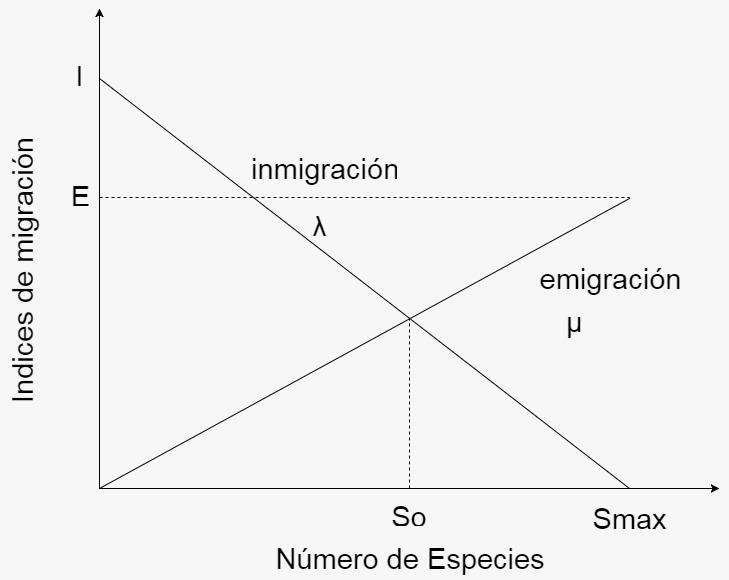
\includegraphics[scale=0.3]{curvaInmEmig.png}
  \caption {Curva de emigracion/inmigración}
\end{figure}

\vspace {3mm}
Ahora consideremos la curva de emigración $\mu$, en donde si no existen
especies en la isla la tasa de emigración es cero, y mientras el número de
especies en la isla va incrementando la tasa de emigración también lo hace,
lo cual quiere decir que a medida que aumenta el número de especies en la
isla, más especies están disponibles para emigrar a islas vecinas. La tasa
máxima de emigración E , ocurre cuando la isla alberga al máximo número
de especies que esta puede soportar.


En resumen, se presentan una serie de diferentes factores que serán las bases de dicho metodo de optimizacion
\begin{itemize}
	\item \textbf{Fitness}: Se utiliza para calcular la calidad de las soluciones. (En nuestro caso la dispersion)
	\item \textbf{$\mu$} : Indice de emigracion de una poblacion en concreto. Esta variable indica cuanto probable va a ser que algun elemento de dicha solucion
	      emigre a otra.
	\item \textbf{$\lambda$} : Indice de inmigracion de una poblacion en concreto. Esta variable indica cuanto probable va a ser que algun elemento de dicha solucion
	      sea reemplazado por un elemento de otra solucion.
  \item \textbf{Isla} : En nuestro caso de trata de una poblacion
	\item \textbf{HSI} : Habitat Suitability Index. índice numérico que representa la
  capacidad de un hábitat de mantener un cierto nivel de población de
  diferentes especies. Se obtiene de la combinación de las diferentes
  variables que afectan a la calidad de vida de las especies que habitan ese
  hábitat.
	\item \textbf{SIV} : Suitability Index Variables. Variables independientes que representan las caracteristicas de habitabilidad de una isla. (En nuestro cada SIV sera cada 
  una de las soluciones de la poblacion)
\end{itemize}

Existen tres mecanismos principales de este algoritmo, los cuales son:
\begin{itemize}
  \item \textbf{Elitismo} : Antes de generar nuevas soluciones se guardan un conjunto de soluciones que sean las mejores.
  Estas soluciones seran introducidas al finalizar por las peores de las nuevas generadas.
  \item \textbf{Migracion} : Se realiza una migracion de una solucion a otra. Por probabilidad los elementos de las mejores soluciones se migran a otras soluciones.
  \item \textbf{Mutacion} : Se realiza una mutacion de una solucion. Por probabilidad se cambia un elemento de una solucion por otro. Se debe conservar la factibilidad
  de las soluciones.
\end{itemize}

\subsection{\normalsize Problema donde se prueba el BBO}\large El problema elegido a abordar en esta practica es el siguiente:
Problema de la mínima dispersión diferencial\textbf{(MDD)}.
Es un problema de optimización combinatoria consistente en
seleccionar un subconjunto M de m elementos (|M|=m) de un conjunto inicial N de n
elementos (con n>m) de forma que se minimice la dispersión entre los elementos
escogidos.

Este problema tiene diferentes \textbf{aplicaciones en el campo de la optimización},
como pueden ser la elección de la localización de elementos públicos, selección
de grupos homogéneos, identificación de redes densas, reparto equitativo, problemas
de flujo, etc

\begin{figure}[h]
	\centering
	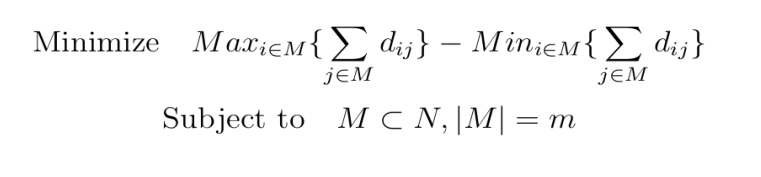
\includegraphics[scale=0.5]{FormulaMinimizacion.png}
\end{figure}

donde:
\begin{itemize}
	\item M es una solución al problema que consiste en un vector binario que indica los m
	      elementos seleccionados
	      \item$d_{ij}$ es la distancia existente entre los elementos i y j.
\end{itemize}

Para resolver este problema se utilizarán 50 casos seleccionados con distancias reales
con, n entre {25,50,75,100,125,150}, y m enttre 2 y 45.

\vspace{5mm}

La Dispersión de una Solución es la diferencia de los valores extremos, es decir,
la diferencia de la sumas de las distancias de dichos puntos al resto de los puntos.
Por ejemplo, si tenemos 8 puntos para colocar farmacias, y solo podemos colocar 4,
\textbf{¿cuál es la forma de colocarlas, de forma que se reduzca la dispersión?}

Los datos se encuentran en unos ficheros \emph{.txt}, donde hay una primera línea
que indica el numero de elementos \emph{n} y el número de elementos a seleccionar
\emph{m} del problema.
\newline Luego se encuentran \textbf{\emph{n*(n-1)/2}} líneas con el formato i,j,$d_{ij}$ que
tienen el contenido de las \textbf{distancias entre los elementos}.
\newline En mi caso, para los dos algoritmos he leido estos ficheros
y he almacenado los datos en una matriz distancias completa, donde la diagonal es 0,
y las triangulares superiores e inferiores son simétricas entre sí.

\vspace{5mm}

La posición (2,3) de la matriz distancias es la distancia entre los elementos 2 y 3,
que a su vez es la misma que la posición (3,2).

\vspace{5mm}

La \textbf{representación de la solución} es un vector de enteros, donde la posición i-ésima
es el numero del elemento que esta seleccionado.
Mantengo en el conjunto de datos solución en la implementación el vector binario usado en la
practica anterior, para la reutilizacion de código.

\vspace{5mm}

Para la \textbf{factorización de la función objetivo}, a la hora de generar una nueva solución no
es necesario volver a calcular por completo el vector de distancias para obtener la nueva
dispersión. Basta con restar la distancia a cada elemento de la solución al elemento que
se ha quitado de la solución actual, y sumarle la distancia del nuevo elemento a todas las demás
de la solución.
\newline Entonces,teniendo el vector de distancias actualizado, para saber la dispersión de dicho conjunto
de elementos restamos la mayor distancia de dicho vector con la menor

\vspace{5mm}

Debido a que se requiere aleatoriedad en ambos algoritmos, ya que son probabilísticos, he usado un vector de semillas,
donde en cada iteración que
realiza cada algoritmo se genera una nueva semilla, y se utiliza para generar nuevas soluciónes.
El valor estático de la semilla sirve para que cada vez que se ejecute el algoritmo, se obtengan las mismas Soluciónes.

También se pedía calcular el tiempo de ejecución de cada algoritmo, por lo que he usado objetos de la clase
\textbf{<chrono>} para tener una alta precisión en los tiempos, y los muestro en \textbf{segundos}.

\vspace{5mm}

Al finalizar cada algoritmo calculo el tiempo demorado por dicho algoritmo y la dispersión de la
mejor solución encontrada.

\vspace{5mm}


\subsection{\normalsize Exploración vs Explotacion}
En BBO no hay algo como una operación de cruce; las soluciones se ajustan
finamente gradualmente mientras el proceso continúa por la operación de
migración. Esto da una ventaja al BBO sobre otras técnicas evolutivas. 
BBO tiene una gran habilidad de explotación en un
problema de optimización global. 

\begin{figure}[h]
  \centering
  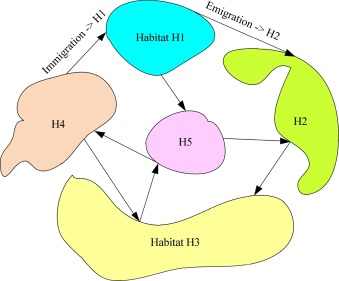
\includegraphics[scale=1]{Islas.png}
  \caption{Islas}
\end{figure}

Para la explotación se van a utilizar las migraciones, que van a consistir en migrar elementos de las mejores
soluciones a las peores. Esto se hace para que las soluciones buenas mejoren a las peores.
Para la exploración se utilizan las mutaciones, que son las que se aplican a todas las soluciones en igual proporción.
Habrá una variable que define con que probabilidad se produce una mutacion. Las mutaciones producen un cambio en la solucion, y se debe buscar un elemento 
nuevo que va a ser el que entre en la solucion por el anterior. 

\subsection{\normalsize Equilibrio}
Este algoritmo presenta muy buen equilibrio entre la exploración y la explotación. Esto se debe a que casi con igual proporcion se van 
a realizar las migraciones y las mutaciones.
Sin embargo, en el problema donde ha sido aplicado el algoritmo la migracion no funciona tan bien como en otros casos, y esto se debe a que 
para ser factible la solucion como hemos comentado antes debe tener un numero exacto de elementos seleccionados. Por lo tanto, cuando se 
realiza la migracion en una solucion, se debe eliminar un elemento de los seleccionados de dicha solucion y esto se hace de forma aleatoria.
Se pueden perder elementos de las soluciones que sean prometedores por la aleatoriedad del algoritmo a la hora del reemplazamiento del elemento de la 
solucion.

En este problema en especifico encontramos una mejor explotacion que exploracion, ya que la exploracion realmente no cambia mucho la solucion, al tener
que encontrar otro elemento que entre en esta para guardar la factibilidad.
En cambio en la explotacion a pesar de que podamos perder un elemento bueno de la solucion, entrará un elemento que probabilisticamente debe ser prometedor
tambien.


\section{\large ADAPTACION DEL BBO AL PROBLEMA DE LA MINIMA DISPERSION DIFERENCIAL}
Para adaptar este algoritmo al problema de la minima dispersion diferencial he tenido que hacer ciertos cambios.\\

Primero el tamanio de la poblacion(numero de islas), viene dado por el tamaño de la poblacion aleatoria generada. \\
Las variables de $\mu$ y $\lambda$ vienes dadas en un vector del mismo tamaño de la poblacion. Por ejemplo para una 
poblacion de tamaño 10 estos serian los valores de $\mu$ y $\lambda$:

\begin{figure}[h]
  \centering
  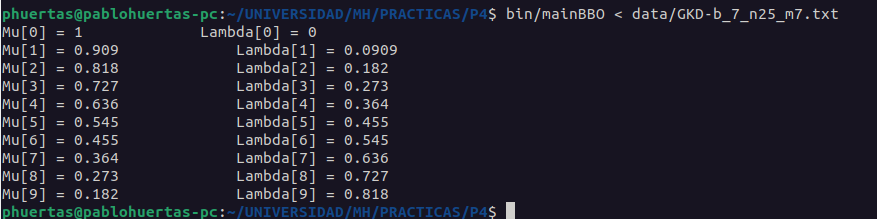
\includegraphics[scale=0.5]{MuLa.png}
  \caption{Valores de $\mu$ y $\lambda$ para un tamaño de poblacion de 10}
\end{figure}

\vspace{3mm}
Ahora toca ordenar la poblacion por fitness, y esto se realiza ordenando de menor a mayor dispersion. \\
Las soluciones con menor dispersion estarán mas arriba en la poblacion. Asi se cumple la relacion 1 a 1 entre el 
vector de $\mu$ y $\lambda$ y la poblacion.\\
Es por esto, que la primera solucion será la mejor, y coincide con el máximo valor de $\mu$ que es 1.\\
Es interesante que esta solucion al ser la mejor comparta sus caracteristicas a las peores, que tendran un valor 
de $\lambda$ elevado.\\

Se genera un conjunto de elites, de tamaño elegido arbitrariamente, por ejemplo 0.1*tamaño de la poblacion si la 
poblacion es minimo de 10 soluciones, o mayor sera este valor si la poblacion es mas pequeña para asegurarnos que hay 
al menos algun elite que se guarda.\\

Ademas vamos a ir almacenando siempre la mejor solucion encontrada. Cada vez que se ordena la poblacion por fitness, se 
comprueba si el primer elemento tiene menor dispersion que la mejor encontrada hasta el momento y si es asi 
se sustituye. Esta solucion sera la solucion final.\\

Luego se entraria en el bucle donde se generan cada una de las generaciones del algoritmo, con dos bucles internos correspondientes 
anidados, uno de 0 hasta el tamaño de la poblacion y otro de 0 hasta el numero de elementos que han de ser seleccionados en 
el caso del problema en concreto.\\

En el bucle más interno es donde se realiza el proceso de migracion, mientras que en el bucle intermedio es donde 
se va a realizar la mutacion con una probabilidad tambien elegida arbitrariamente.\\

El proceso de mutacion se podria meter dentro del bucle más interno, pero habria que disminuir 
la probabilidad de mutacion ya que se ejecutarían muchas más mutaciones de las que deseamos.\\
De todas formas esto es un parametro muy arbitrario, ya que el valor que asignemos a la probabilidad de mutacion va 
a depender mucho de si queremos una mayor explotacion o menor.\\

Cada vez que se migra o muta un elemento, se calcula la funcion objetivo de la solucion modificada.\\

\vspace{3mm}
\begin{algorithm}
	\normalsize
	\label{Algoritmo BBO}
	\caption{Algoritmo de Optimizacion Basada de Biogeografia}
	\KwIn{$n, m , poblacion, prob_{mutacion}, n_{generaciones}, n_{elites} $}
	\KwOut{$solucion$}

	$poblacion \leftarrow \emph{(ORDENAR \ POR \ FITNESS)}$\\
	\vspace{1mm}
	$mu \leftarrow \{ \mathbf{1}, \ldots, \mathbf{0} \}$\\
	$lambda \leftarrow \{ \mathbf{0}, \ldots, \mathbf{1} \}$\\
	\vspace{3mm}

	$mejor_{solucion} \leftarrow \mathbf{poblacion[0]}$\\

	\vspace{3mm}
	$Vector Distancias \leftarrow{\emph{GenerarVectorDistancias()}}$\\
	$Dispersion Comparacion \leftarrow{\emph{Calculardispersion(VectorDistancias)}}$\\
	\vspace{3mm}
	$Mejora \leftarrow {\textbf{TRUE}}$\\
	\vspace{3mm}
	\For{$n_{iteraciones} \in n_{generaciones}$}{
		$elites \leftarrow \{ \mathbf{poblacion[0]}, \ldots, \mathbf{poblacion[n_{elites}]} \}$\\
		\vspace{3mm}
		\For{$i \in Size(poblacion)$}{
			\For{$j \in m$}{
				\If{$Random.Get(0,1) \leq \mathbf{lambda[i]}$}{
					$\mathbf{poblacion[i] \leftarrow \emph{MIGRACION}}$\\
					$\mathbf{poblacion[i] \leftarrow \emph{RECALCULAR \ FUNCION \ OBJETIVO}}$\\
				}
			}
			\If{$Random.Get(0,1) \leq \mathbf{prob_{mutacion}}$}{
				$\mathbf{poblacion[i] \leftarrow \emph{MUTACION}}$\\
				$\mathbf{poblacion[i] \leftarrow \emph{RECALCULAR \ FUNCION \ OBJETIVO}}$\\	
			}
		}

		$poblacion \leftarrow \emph{(ORDENAR \ POR \ FITNESS)}$\\
		$poblacion \leftarrow \emph{(SUSTITUIR \ PEORES \ POR \ ELITES)}$\\
		\vspace{3mm}
		\If{$mejor_{solucion}.dispersion < \mathbf{poblacion[0].dispersion}  $}{
			$mejor_{solucion} \leftarrow \mathbf{poblacion[0]}$\\
		}
		\vspace{3mm}
	}

	$return \{ mejor_{solucion}\}$
\end{algorithm}


\vspace{5mm}



\subsection{\large Descripción de la función objetivo}
La función objetivo de este problema es la de encontrar la dispersión a partir de un vector de
booleanos donde la posición i-ésima es 1 si el elemento i-ésimo está seleccionado, y 0 en caso contrario.\\
Para evaluar la función objetivo, se convierte internamente el vector de booleanos en una selección
de elementos de números enteros.\\
Para ello, se recorre el vector de booleanos, y si la posición i-ésima es 1, se añade al final del vector de
seleccionados el elemento i-ésimo.\\
Tenemos la matriz de distancias comentada anteriormente, y la selección de elementos, por lo
que para evaluar la función objetivo, para cada elemento del vector de seleccionado, en la posición i-ésima
del vector distancias, añadimos la distancia del elemento i-ésimo a todos los demás elementos del vector de seleccionados.\\
Las posiciones se corresponden 1 a 1 en los vectores de seleccionados y distancias.
\vspace{5mm}

\begin{algorithm}
	\scriptsize
	\label{Algoritmo de Evaluacion de la Funcion Objetivo}
	\caption{Algoritmo de Evaluación de la Función Objetivo}
	\KwIn{distancias(vector), seleccionados(vector), m(matriz distancias)}% Parámetros de entrada
	$distancias \leftarrow 0$\\

	\vspace{3mm}

	\vspace{3mm}
	$Vector Distancias \leftarrow{\emph{GenerarVectorDistancias()}}$\\
	$Dispersion Comparacion \leftarrow{\emph{Calculardispersion(VectorDistancias)}}$\\
	\vspace{3mm}
	$Mejora \leftarrow {\textbf{TRUE}}$\\

	\For{$i \in Size(seleccionados)$}{
		$a comparar \leftarrow i $\\
		\For{$j \in Size(seleccionados)$}{
			\If{$seleccionados[i] \neq acomparar$}{
				$distancias[i] += m[acomparar][seleccionados[i]]$\\
			}
		}
	}
\end{algorithm}

\subsection{\normalsize Descripción de los operadores comunes}
Hay ciertos operadores y funciones que son comunes para los algoritmos desarrollados en esta práctica,
ya que por ejemplo la generación de soluciónes aleatorias es común y varios operadores
más, por lo que voy a desglosar uno a uno para entrar más en profundidad.

\vspace{3mm}

\subsubsection{\small Generación de soluciones aleatorias}
Para la generación de la primera solución aleatoria, utilizo una funcion para generar soluciónes
aleatorias, donde el numero de posibles elementos a escoger es emph{n} y el numero que finalmente son seleccionados
son emph{m}.

\begin{algorithm}
	\label{Algoritmo de Generacion de soluciones Aleatorias}
	\caption{Algoritmo de Generación de soluciónes Aleatorias}
	\KwIn{n(número de puntos) m(número de puntos a seleccionar), semilla(número que simboliza una semilla estática) }% Parámetros de entrada
	\KwOut{solución(vector de booleanos)}% Parámetros de salida
	\vspace{3mm}

	$solución \leftarrow \emptyset $\\
	$seleccionados \leftarrow \emptyset $\\
	\vspace{3mm}

	\While{$Size(seleccionados) < m$}{
		$seleccionados \leftarrow \emph{Numero aleatorio que no esta en seleccionados} $\\
		$solución \leftarrow \emph{seleccionados.back} $\\
	}
\end{algorithm}

\vspace{3mm}




\newpage
\section{\large PROPUESTA DE MEJORA DE LA METAHEURISTICA}

Como propuesta de mejora del algoritmo BBO, he decidido usar un operador de reparacion de las soluciones, ya que como hablamos antes hay soluciones
que al migrar o al mutar pueden perder la factibilidad. Este operador de reparacion tiene como objetivo no volver a hacer factible la solucion de forma aleatoria tal y como estabamos haciendo,
sino que tener en cuenta al eliminar el o los elementos que sobran o introducir los que faltan teniendo en cuenta cuanto se aleja su fitness(dispersion) a la media de las dispersiones 
de la solucion actual.\\
Es decir, el eliminar elementos de la solucion se eliminaran los que tengan un fitness mas alejado de la media de fitness de dicha solucion, e igual al introducir un elemento, que se tendra en cuenta 
con que valor queda la media de fitness con ese elemento en la solucion. Por lo tanto para introducir un elemento se introducira el que menos aumente la dispersion (o la reduzca), mientras que al eliminar un 
elemento bastará con eliminar el que tenga el fitness mas alejado de la media de fitness de la solucion(ya sea por encima o por debajo). 

\subsection{\normalsize Hibridacion con \\Enfriamiento Simulado}

Una tecnica de mejora del algoritmo es la Hibridacion con Enfriamiento Simulado.\\
Este algoritmo se lo aplico a las soluciones que pueden estar mas estancadas en un optimo local, ya que sabemos que el algoritmo de Enfriamiento simulado tiene 
buenas tecnicas de escape de estos optimos. Por lo tanto lo aplico por defecto a todas las soluciones cada 5 generaciones para que haya una exploracion mas pronunciada.

A continuacion se muestra una descripcion del algoritmo de Enfriamiento Simulado
\subsubsection{\scriptsize Algoritmo de Enfriamiento Simulado}
El algoritmo de Enfriamiento Simulado \emph{(Simulated Annealing)} es un algoritmo de búsqueda metaheuristica
para problemas de optimización global.\\
El objetivo de este algoritmo es encontrar una solución optima o casi optima de un problema en un espacio
de búsqueda grande.\\
Tiene un criterio probabilistco de aceptacion de soluciónes basado en Termodinamica.\\
La forma que tiene de escapar de óptimos locales, es la posibilidad de aceptar soluciónes peores con una cierta probabilidad,
la cual va disminuyendo conforme se va avanzando en el algoritmo hacia una buena solución.\\
Tiene una filosofía de diversificar al principio e intensificar al final, es decir, al principio del algoritmo
se evaluan multiples soluciónes distintas y se selecciona la mejor, y al final se intensifica la búsqueda
explotandola.
\vspace{5mm}

El máximo de éxitos que se podrán generar como máximo en cada iteracion del algoritmo serán n.\\
El máximo de vecinos que se podrán generar como máximo en cada iteracion del algoritmo serán 10*n.\\
La constante $\mu$ tendra valor 0.3 en toda la ejecucion \\
La temperatura inicial se calculará como...
\begin{equation}
	\emph{To} = \frac{ \mu * C(So)  }{ - \ln( \varphi  )   }
\end{equation}
\newline siendo $\varphi$ = $\mu$

\vspace {5mm}
Beta se calculará de la forma...
\begin{equation}
	\beta = \frac{ t_i - t_f }{ t_i * t_f * n  }
\end{equation}
\newline siendo $t_i$ la temperatura inicial, $t_f$ la temperatura final y $n$ el tamaño de la solución.
\vspace {5mm}

Al final de cada iteracion se calcula la temperatura que se va a tomar como nueva, y esta
se calcula de la forma...
\begin{equation}
	t_{k1} = \frac{ t_k }{ 1 + (\beta * t_k) }
\end{equation}
\newline siendo $t_k$ la temperatura actual y $k$ el numero de iteracion.

El número máximo de evaluaciones de la funcion objetivo del algoritmo completo serán \textbf{100000}

\begin{algorithm}[h]
	\scriptsize
	\label{Algoritmo de Enfriamiento Simulado}
	\caption{Algoritmo de Enfriamiento Simulado}
	\KwIn{ TemperaturaInicial(temperatura inicial), TemperaturaFinal(temperatura final)}% Parámetros de entrada
	\KwOut{ TemperaturaActual(temperatura actual) }% Parámetros de salida
	\vspace{3mm}

	$TemperaturaInicial \leftarrow CalcularTemperaturaInicial(\mu, \varphi, C(S_o))$\\
	$TemperaturaActual \leftarrow TemperaturaInicial $\\
	$TemperaturaFinal \leftarrow 10^{-3} $\\
	$nEnfriamientos \leftarrow  1000/n$\\
	$maxVecinos \leftarrow 10*n$\\
	$maxExitos \leftarrow n$\\
	\vspace {3mm}
	$iteraciones \leftarrow 0$\\
	$evaluaciones \leftarrow 0$\\
	$s_o \leftarrow \emph{CalcularsoluciónAleatoria}$\\
	$s_{mejor} \leftarrow S_o$\\
	\vspace {3mm}
	\While{$(TemperaturaActual > TemperaturaFinal) \&\& (iteraciones < nEnfriamientos) \&\& (nEvaluaciones < 100000)$}{
		$exitos \leftarrow 0$\\
		\For{$i \in 1 \ldots maxVecinos \ \&\& \ exitos < maxExitos$}{
			$S_{Vecino} \leftarrow GenerarsoluciónVecinaAleatoria()$\\
			$evaluaciones \leftarrow evaluaciones + 1$\\

			\vspace {3mm}
			$\Delta_{dispersion} \leftarrow dispersion(S_{vecino}) - dispersion(S_{actual})$\\

			$\emph{Calculamos la probabilidad de que se acepte la nueva si es peor que la actual}$\\
			$probabilidad \leftarrow e^{-\Delta_{dispersion} / TemperaturaActual}$\\

			\vspace {3mm}
			\If{$ (\Delta_{dispersion} <  0 ) \ or \ (GetRandomNumber(0,1) < probabilidad) $}{
				$S_{actual} \leftarrow S_{vecino}$\\
				$exitos \leftarrow exitos + 1$\\
			}

			\vspace {3mm}

			\If{$dispersion(S_{actual}) - dispersion(S_{mejor})$}{
				$S_{mejor} \leftarrow S_{actual}$\\
			}

		}
		$beta \leftarrow \emph{CalcularBeta}$\\
		$TemperaturaActual \leftarrow CalcularTemperaturaActual(t_k, \beta, t_i, n)$\\
		$iteraciones \leftarrow iteraciones + 1$\\
	}

	$return \ S_{mejor}$

\end{algorithm}




\subsubsection{\scriptsize Operador de mutacion}
La mutacion consiste en modificar con cierta probabilidad uno o varios genes de la poblacion (en este caso de una solución)
aleatoriamente. La probabilidad de mutacion es dada por la constante \emph{probabilidad 0.1}.
Cuando muta un gen de un cromosoma, tenemos que encontrar otro gen del mismo cromosoma con el valor contrario,
para mantener la factibilidad de la solución de dicho cromosoma.
Por ejemplo, en una solución con 10 elementos donde se seleccionan 3, si se va a mutar el segundo seleccionado, tenemos que buscar uno de los 7
elementos que no esten seleccionados de manera aleatoria y cambiar el valor de cada gen.
El rango de elementos que pueden ser mutados, van desde 0 hasta el producto del numero de cromosomas por el numero de genes
por cromosoma.\\
Si la poblacion tiene 10 cromosomas, y cada cromosoma 5 genes, si se genera para mutar el elemento 15, será el sexto gen del segundo cromosoma.

\begin{algorithm}[H]
	\scriptsize
	\label{Operador de Mutacion}
	\caption{Operador de Mutación}
	\KwIn{ p(poblacion), prob(probabilidad) }% Parámetros de entrada
	\KwOut{ pnueva(poblacion generada) }% Parámetros de salida
	\vspace{3mm}

	$rango$ $mutacion \leftarrow \emph{p.NumeroDeCromosomas()} \cdot \emph{p.NumeroDeGenesPorCromosoma()} $\\

	\For{$i \in Size(p)$}{
		\If{$GenerarNumeroAleatorioEntre(0,1) < prob$}{
			$\emph{Genero aleatoriamente un elemento en el rango de mutacion}$\\
			$posicion \leftarrow GenerarNumeroAleatorioEntre(0,rango) $\\

			$\emph{Para el elemento de la posicion generada, busco otro gen del mismo cromosoma
					con el valor contrario}$\\
			$posicion2 \leftarrow \emph{Gen del mismo cromosoma aleatorio con valor contrario} $\\

			$\emph{Swap(posicion, posicion2)}$\\
		}

	}
	$return$ $pnueva$\\

\end{algorithm}
\vspace {3mm}

En la ejecucion del algoritmo se realizan 10 iteraciones y cada BL como máximo hara \textbf{10000} evaluaciones
o no mejore la solución en todo el entorno.
El valor usado para el numero de genes a mutar de la solución es \emph{t = 0.3}

\newpage
\subsection{\normalsize Hibridacion con \\ Busqueda Local}
Anteriormente hemos visto una posible hibridacion con el algoritmo de Enfriamiento Simulado.\\
Ahora vamos a ver una hibridacion con la busqueda local. Sabemos que el algoritmo de Busqueda Local
tiene una explotacion muy pronunciada, por lo que si lo combinamos con un algoritmo con buena exploracion como es 
el BBO en nuestro caso (que hemos visto que para este problema la explotacion no es su punto fuerte por la propia estructura de la funcion objetivo)
podemos obtener muy buenos resultados y vamos a experimentar sobre ello.

A continuacion se muestra una descripcion del algoritmo de busqueda local.

\subsubsection{\scriptsize Busqueda Local}
Este algoritmo es un tipo de algoritmos de busqueda por trayectorias simples.
\newline En este algoritmo, se empieza con una solución inicial completa y aleatoria,
es decir, una Solución con \emph{M} elementos que no se repiten entre sí.
El orden de estos elementos no es relevante.
\vspace{5mm}
%o Para el algoritmo BL, el métodos de exploración del entorno, el operador
%de generación de vecino, la factorización de la BL y la generación de
%Soluciónes aleatorias.
\newline La idea es tras haber generado una completa Solución aleatoria válida, generar el
\textbf{vecindario completo} de la Solución actual, \textbf{desordenarlo aleatoriamente}, y recorrerlo
comparando en cada iteracion si se mejora la Dispersión.
\newline Si se mejora la Dispersión, se \textbf{selecciona dicha Solución como Solución actual} y
se vuelve a generar el vecindario. Este proceso se hace hasta que no se mejore la Dispersión con
todo el vecindario generado o hasta que se hayan hecho \textbf{100000 evaluaciones de la funcion objetivo}.
Es decir, comprobar 100000 veces si se mejora la Dispersión.
\newline Como vemos este algoritmo se parece a Greedy en que ambos cuando encuentran una Solución
mejor que la anterior la seleccionan, y no se espera en este caso a recorrer todo el vecindario para
encontrar una mejor Solución. Es por eso que este algoritmo se llama Busqueda Local de \textbf{Primero el mejor}
\vspace{5mm}
\newline La generación de la primera Solución aleatoria se hace con un bucle que va generando
numeros aleatorios entre 0 y n-1, de forma que si no se ha añadido aún a la Solución, lo añade.
Este proceso se repite hasta que el numero de elementos de la Solución sea igual a \emph{M}
\newline Para la generación de vecinos, uso un vector de tuplas, que contienen el elemento que se
va a intercambiar y el elemento que se va a intercambiar y va a entrar a la Solución provisional.
\newline Por ejemplo, si tengo {M}=6 y {N}=3, Solución provisional=(1,3,5), y genero el vecindario de esta Solución,
este será el vector de tuplas \newline {(1,0), (1,2) ,(1,4), (3,0), (3,2), (3,4), (5,0), (5,2), (5,4)}.
\newline Entonces, desordena este vector aleatoriamente y se va intercambiando la posicion primera
de la tupla que se encuentra en la Solución por la segunda posicion de la tupla que no se encuentra en la Solución
\newline La factorización es la misma que en el algoritmo greedy, cuando se intercambia un elemento de la Solución
por otro, en el vector distancias a cada elemento se le resta la distancia con el elemento que se elimina,
y se le suma la distancia con el elemento que se añade, ademas de añadir en la posicion del elemento añadido
la distancia con todos los demas de la Solución.

\vspace{10mm}
\newpage
\maketitle \textbf{PSEUDOCÓDIGO DEL ALGORITMO DE BUSQUEDA LOCAL}
\begin{algorithm}[H]
	\scriptsize
	\label{Algoritmo Busqueda Local}
	\caption{Algoritmo de búsqueda local}
	%\KwIn{n, m, solución}% Parámetros de entrada
	$v \leftarrow 0 $,$ w\leftarrow 0 $\\
	$ S\leftarrow D $\\
	$T \leftarrow \emptyset $\\
	$solución \leftarrow \emptyset$\\
	$Elementos restantes \leftarrow V$\\
	$Dispersion Comparacion \leftarrow \emptyset$\\
	$Distancias \leftarrow \emptyset$\\
	$Dispersion \leftarrow \emptyset$\\
	\vspace{3mm}
	$Copia solución \leftarrow \emptyset$\\
	$Copia Distancia \leftarrow \emptyset$\\
	$Vecindario \leftarrow \emptyset$\\
	\vspace{3mm}
	\While{$solución < M$}{
	\vspace{1mm}
	$\emph{Vamos generando elementos aleatorios y los introducimos a la solución}$\\
	$Elemento a introducir \leftarrow{\emph{GenerarElementoAleatorio(Elementos restantes)}}$\\
	$Elementos restantes \leftarrow{Elementos restantes-{Elemento a introducir}}$\\
	$solución \leftarrow{solución \cup {Elemento a introducir}}$\\
	}
	$\emph{Ya tenemos una solución completa y válida de tamaño M}$\\
	$\emph{El conjunto de elementos restantes solo contiene}$\\
	$\emph{los elementos que no están en la solución}$\\
	\vspace{3mm}
	$Vector Distancias \leftarrow{\emph{GenerarVectorDistancias()}}$\\
	$Dispersion Comparacion \leftarrow{\emph{Calculardispersion(VectorDistancias)}}$\\
	\vspace{3mm}
	$Mejora \leftarrow {\textbf{TRUE}}$\\

	\While{Mejora == TRUE {\&\&} iteraciones \textbf{$\leq$} 100000}{
		$\emph{Generamos un vecindario completo de la solución actual}$\\
		$\emph{ y lo mezclamos aleatoriamente}$\\
		$Vecindario \leftarrow {\emph{GenerarVecindario(solución)}}$\\
		$Vecindario \leftarrow {\emph{Desordenar(Vecindario)}}$\\
		\vspace{3mm}
		$\emph{Actualizamos las variables antes de recorrer el vecindario}$\\
		$Copia solución \leftarrow{solución}$\\
		$Mejora \leftarrow {\textbf{FALSE}}$\\
		$dispersion comparacion \leftarrow{Dispersion}$\\
		\vspace{3mm}
		\For{$i \in Size(Vecindario) {\&\&} mejora == FALSE $}{
			$\emph{Recorremos el vecindario}$\\
			$Copia solución \leftarrow{\emph{SustituirPunto(vecindario[i])}}$\\
			$Copia Distancias \leftarrow{\emph{GenerarVectorDistancias(Copiasolución)}}$\\
			$dispersion comparacion \leftarrow{\emph{Calculardispersion(CopiaDistancias)}}$\\
		}

		\eIf{dispersion comparacion < dispersion}{
			$\emph{Si la dispersion es mejor, actualizamos la solución}$\\
			$dispersion \leftarrow{\emph{dispersion comparacion}}$\\
			$solución \leftarrow{\emph{Copiasolución}}$\\
			$Mejora \leftarrow{\textbf{TRUE}}$\\
			$VectorDistancias \leftarrow{\emph{CopiaDistancias}}$\\
			$Restantes \leftarrow{\emph{CalcularRestantes(solución)}}$\\
		}{
			$\emph{Si la dispersion no es mejor, no actualizamos la solución,}$\\
			$\emph{y volvemos al estado anterior}$\\
			$Copia solución \leftarrow{solución}$\\
			$Copi Distancias \leftarrow{Vector Distancias}$\\
		}

		$Iteraciones \leftarrow{\emph{Iteraciones}+1}$\\
	}

	$\emph{Devolvemos la solución}$\\
	$\textbf {Return solución}$\\

\end{algorithm}

\newpage

\newpage
\section{\large ESTUDIO EXPERIMENTAL Y ANÁLISIS \\DE RESULTADOS}
En ambos algoritmos hemos usado el mismo vector de semillas, que en cada iteración
que ejecuta el programa el algoritmo, se coge la posicion i-esima del vector de semillas.
\newline El vector semillas es (1,2,3,4,5)
Por lo tanto en la primera iteracion se define la semilla como Random::Seed(1), y asi
sucesivamente.
\newline Para comparar los resultados entre los dos algoritmos implementados en esta práctica, he hecho
una tabla donde se muestran, para cada algoritmo, el tiempo medio y la dispersion media conseguida entre
las 5 iteraciones conseguido con cada uno de los ficheros de datos.

\vspace{10mm}
\begin{figure}[h]
	\centering
	\subfloat[Tabla de resultados de Greedy]{
		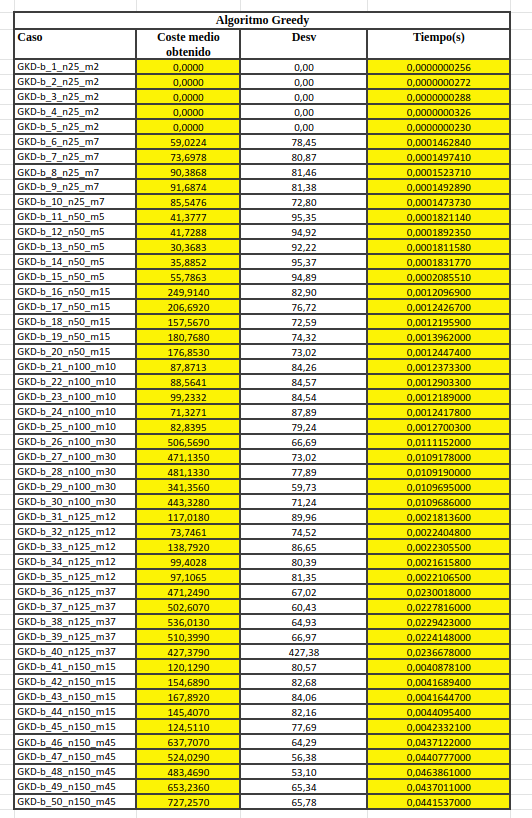
\includegraphics[width=0.3\textwidth]{TablaGreedy.png}}
	\subfloat[Tabla de resultados de BL]{
		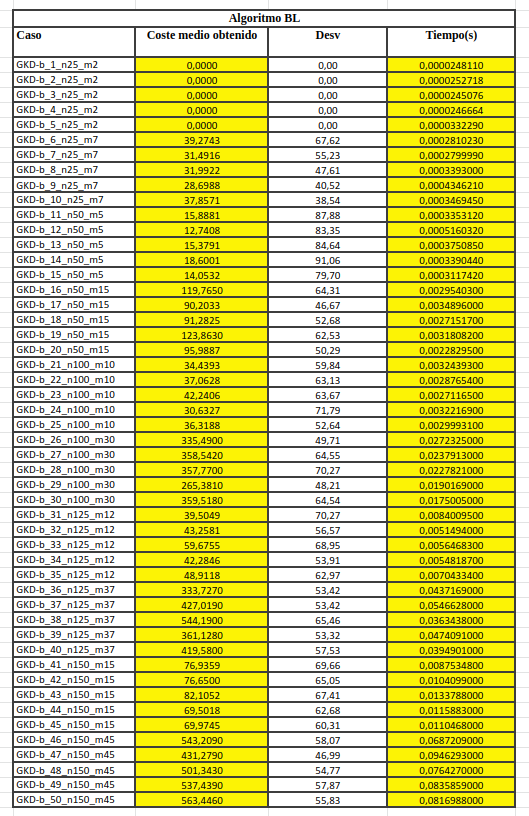
\includegraphics[width=0.3\textwidth]{TablaBL.png}}
	\caption{Tablas de resultados de Greedy y BL}
\end{figure}

\begin{figure}[h]
	\centering
	\subfloat[Desviacion y tiempo de Greedy]{
		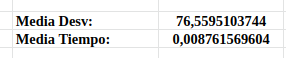
\includegraphics[width=0.3\textwidth]{DesvGreedy.png}}
	\subfloat[Desviacion y tiempo de BL]{
		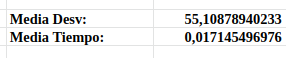
\includegraphics[width=0.3\textwidth]{DesvBL.png}}
	\caption{Desviaciones y tiempos de Greedy y BL}
\end{figure}

\vspace{10mm}
Observando los datos de las tablas, podemos observar que el algoritmo greedy tiene un
tiempo menor que busqueda local, mientras que tiene una mayor desviacion, lo que quiere decir
que sus resultados de dispersiones son peores.
\vspace{10mm}

Aunque estas diferencias no sean muy significativas, a la hora de evaluar muchas ejecuciones
de estos algoritmos, encontramos como se acentúa más la diferencia.
\vspace{5mm}

\vspace{10mm}
\begin{equation}
	\textbf{Desviacion} =
	100*\sum_{i=1}^n
	\frac{ValorAlgoritmo_i - MejorValor_i}{ValorAlgoritmo_i}
\end{equation}

\vspace{10mm}
Por lo tanto, tenemos unos datos de referencia, que contienen el mejor coste obtenido para
cada instancia del problema.
El algoritmo de Busqueda Local obtiene mejores dispersiones de media que Greedy, y esto es gracias a que
este algoritmo tiene mas probabilidad de encontrar mejores soluciónes.
\newline Al generar el vecindario completo se asegura que si no se encuentran mejores
dispersiones, no las selecciona, al contrario que Greedy, que aunque ninguno mejore la dispersion
añade a la solución el que menos la empeore.
\newline Esto evita que el algoritmo de Busqueda Local vaya hacia soluciónes peores(mínimos locales), y siempre
se asegure que cuando actualiza la solución es para una mejor dispersion.
\newpage En cambio, Greedy acepta soluciónes peores a la actual, y esto puede hacer que caiga en mínimos locales,
y al siempre añadir elementos a la solución, no poder salir de ellos.

\begin{figure}[h]
	\centering
	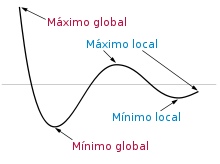
\includegraphics[scale=0.5]{MinLocal.png}
	\caption{Gráfica que muestra el comportamiento de una búsqueda de una solución}
\end{figure}


\subsection{Tabla resumen}
\begin{table}[h]
	\begin{center}
		\begin{spacing}{1.5}
			\begin{tabular}{| l | l | l | }
				\hline
				\textbf{Algoritmo}    & \textbf{Desviación media} & \textbf{Tiempo (en segundos)} \\ \hline
				\emph{Greedy}         & 76,5595103744             & 0,008761569604                \\ \hline

				\emph{BL}             & 55,10878940233            & 0,017145496976                \\ \hline

				\emph{AGG-Uniforme}   & 40,0088991109             & 7,463298200000                \\ \hline

				\emph{AGG-Posición}   & 45,4862646141             & 3,312911800000                \\ \hline

				\emph{AGE-Uniforme}   & 55,9744088626             & 9,524131200000                \\ \hline

				\emph{AGE-Posición}   & 54,5438597140             & 5,062808200000                \\ \hline

%				\emph{AM-(10,1.0)}    & -0,0978477902             & 35,944350200000               \\ \hline
%
%				\emph{AM-(10,0.1)}    & 14,6659436747             & 6,939745800000                \\ \hline
%
%				\emph{AM-(10,0.1mej)} & 32,5667149186             & 5,862021000000                \\ \hline
				
				\emph{ES} & 39,6364925123 & 0,019224743220 \\ \hline
				\emph{BMB} & 35,4212565508 & 0,239388720600 \\ \hline
				\emph{ILS} & 38,7884380920 & 0,100818801540 \\ \hline
				\emph{ILS\_ES} & 39,6364925123  & 0,019224843220 \\ \hline 

				\emph{BBO}			& 42,0759918345          & 0,455122914000               \\ \hline

				\emph{BBO-BL}		& 20,5689749201             & 0,324748746000               \\ \hline

				\emph{BBO-BL+}	& 10,3153847989 		   & 8,397473508000               \\ \hline
			
			\end{tabular}
		\end{spacing}
		\caption{Tabla de medias de desviaciones y tiempos de los algoritmos}
	\end{center}
\end{table}


\newpage
\subsection{Analisis resultados BBO}
A continuacion voy a analizar los resultados de BBO, con todas las variantes realizadas en el
\subsubsection{BBO sin hibridacion}
En la primera prueba del algoritmo hemos visto que nos da dispersion 42, con un tiempo bastante bueno y con los siguientes parametros:
\begin{itemize}
	\item{Tamaño de poblacion : 100}
	\item{Numero de iteraciones : 200}
	\item{Probabildad de mutacion : 0.1}
	\item{Numero de elites : 20}
\end{itemize}
\vspace{3mm}
Observamos que tenemos parametros bastante generosos, lo que va a permitir bastante la exploracion, ya que como hemos 
comentado anteriormente el BBO en nuestro problema de optimizacion, no tiene una gran calidad de explotacion 
debido a la propia naturaleza de la funcion objetivo, por lo que hemos decidido probar a explorar de una forma 
mas exhaustiva, es decir, con una poblacion de tamaño mayor y mayor probabilidad de mutacion.

\vspace{3mm}
\subsubsection{BBO con hibridacion BL}
En esta hibridacion con la Busqueda Local hemos usado los siguientes parametros:
\begin{itemize}
	\item{Tamaño de poblacion : 50}
	\item{Numero de iteraciones : 100}
	\item{Probabildad de mutacion : 0.01}
	\item{Numero de elites : 5}
\end{itemize}

\vspace{3mm}
Observamos una muy buena desviacion obtenida de media y un mejor tiempo que en el caso anterior, este se debe a que hemos 
disminuido bastante el numero de iteraciones(numero de generaciones maximo que se van a generar) y el tamaño de la poblacion.\\
Aprovechamos mejor la alta exploracion que presenta el BBO, para posteriormente aplicar una BL sobre la poblacion final.\\
Solo aplicamos dos BL, antes de empezar el BBO y al finalizar.

\vspace{3mm}
\subsubsection{BBO con hibridacion BL++}
En esta hibridacion con la Busqueda Local hemos usado los siguientes parametros:
\begin{itemize}
	\item{Tamaño de poblacion : 100}
	\item{Numero de iteraciones : 50}
	\item{Probabildad de mutacion : 0.1}
	\item{Numero de elites : 5}
\end{itemize}

\vspace{3mm}
Observamos la mejor dispersion media hasta el momento y esto se debe a lo que comentamos anteriormente, de que 
aprovechamos el BBO para una exploracion exhaustiva y aqui aplicamos BBO a todos los elementos de la poblacion en 
cada iteracion. Es por esto que obtenemos los mejores resultados por el momento.

\vspace{3mm}
\subsubsection{BBO con hibridacion ES}
En esta hibridacion con el Enfriamiento Simulado hemos usado los siguientes parametros:
\begin{itemize}
	\item{Tamaño de poblacion : 100}
	\item{Numero de iteraciones : 50}
	\item{Probabildad de mutacion : 0.1}
	\item{Numero de elites : 5}
\end{itemize}

\vspace{3mm}
Observamos que la hibridacion con Enfriamiento Simulado no ofrece malos resultados, pero bastante peores que 
las hibridaciones con BL. Esto se puede deber a que el algoritmo de Enfriamiento Simulado con 10000 evaluaciones de la funcion 
objetivo(que es el ES usado) no llega a explotar bien las soluciones, entones estamos hibridando un algoritmo que explora 
mucho como es el BBO, y otro que en nuestro caso tambien esta explorando mucho, por lo que no se puede conseguir una buena
explotacion final y es por esto que los resultados no son tan buenos.


\end{document}